\section{Часть 4 -- "Цепная".}

\section{Цепные дроби.}

Вернёмся к алгоритму Евклида и посмотрим, что происходит с дробью $\dfrac{a}{b}$ в процессе нахождения наибольшего общего делителя.


$\dfrac{a}{b} = \dfrac{bq_0 + r_1}{b} = q_0 + \cfrac{r_1}{b} = q_0 + \cfrac{1}{\cfrac{b}{r_1}} = q_0+\cfrac{1}{\cfrac{r_1q_1 + r_2}{r_1}} = q_0 + \cfrac{1}{q_1 + \cfrac{1}{\cfrac{r_1}{r_2}}} = \cdots = q_0 + \cfrac{1}{q_1 + \cfrac{1}{q_2 + \cfrac{1}{q_3 + \cdots \cfrac{1}{q_{n - 1} + \cfrac{1}{q_n}}}}}$

\noindent Представление дроби $\dfrac{a}{b}$ в таком виде называется \textit{цепной дробью}.

\underline{\textit{Обозначение:}} $\dfrac{a}{b} = [q_0; q_1, q_2, \cdots, q_n]$ -- если дробь конечна и $\dfrac{a}{b} = [q_0; q_1, q_2 , \cdots]$ -- если дробь бесконечна.

\begin{dfn} 
    \textit{Цепная дробь} (или \textit{непрерывная}) -- это математическое выражение вида $[q_0; q_1, q_2, \cdots] = q_0 + \cfrac{1}{q_1 + \cfrac{1}{q_2 + \cfrac{1}{q_3 + \cdots}}}$, где $q_0$ -- целое число, а остальные $q_i$ -- натуральные. 
\end{dfn} 

\noindent Очевидно, что таким образом можно представить любое действительное число можно представить цепной дробью (конечной или бесконечной).

\begin{thm}
    Докажите, что число представляется конечной цепной дробью тогда и только тогда, когда это число рационально.
\end{thm}

\noindent Если в какой-то момент «оборвать» непрерывную дробь, то можно получить конечную дробь, после преобразований сводящуюся к обыкновенной дроби. Такие дроби называются \textit{подходящими}.

Например, $2 + \cfrac{1}{3 + \dfrac{1}{4}} \left(= \dfrac{30}{13} \right), 5 + \cfrac{1}{1 + \cfrac{1}{3 + \dfrac{1}{2}}} \left(= \dfrac{52}{9}\right).$

Введём обозначения: 
\par $\dfrac{q_0}{1} = \dfrac{P_0}{Q_0}; q_0 + \dfrac{1}{q_1} = \dfrac{P_0}{Q_0}; q_0 + \cfrac{1}{q_1 + \dfrac{1}{q_2}} = \dfrac{P_2}{Q_2}; \cdots q_0 + \cfrac{1}{q_1 + \cfrac{1}{q_2 + \cfrac{1}{{ \substack{q_3 + \cdots\\[1pt]\cdots \cfrac{1}{q_n}}  }} } } = \dfrac{P_n}{Q_n}; \cdots$

\begin{figure}[H]
    \begin{minipage}{0.8\linewidth}
        \begin{thm}
            Представьте число $\dfrac{987}{654}$ виде цепной дроби.
        \end{thm}
        
        \begin{thm}
            Выразите отношение сторон прямоугольного поля, разбитого на квадратные участки (план изображён на рисунке), через цепную дробь.
        \end{thm}
        
        \begin{thm}
            Выразите $\dfrac{P_k}{Q_k} - \dfrac{P_{k - 1}}{Q_{k - 1}}$ и $\dfrac{P_k}{Q_k} - \dfrac{P_{k - 2}}{Q_{k - 2}}$ через $q_0, q_1, \cdots, q_n$. 
        \end{thm}
    \end{minipage}
\hfill
    \begin{minipage}{0.19\linewidth}
        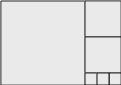
\includegraphics[width=0.95\columnwidth]{img/11.3 img1.png}
    \end{minipage}
\end{figure}

\begin{center}
    \fbox{\begin{varwidth}{\linewidth}
            \begin{thrm}
                («Свойство вилки»).
                \begin{center}
                      $\dfrac{P_1}{Q_1} > \dfrac{P_3}{Q_3} > \cdots > \dfrac{P_{2i - 1}}{Q_{2i - 1}} > \cdots$
                      \par
                      $\dfrac{P_0}{Q_0} < \dfrac{P_2}{Q_2} < \cdots < \dfrac{P_{2k}}{Q_{2k}} < \cdots$
                      \par
                      $\dfrac{P_{2i - 1}}{Q_{2i - 1}} > \dfrac{P_{2k}}{Q_{2k}} (i = 1, 2, \cdots; k = 0, 1, \cdots)$
                  \end{center}
            \end{thrm}
        \end{varwidth}}    
\end{center}


\begin{center}
    \textbf{Замечания к алгоритму Евклида для программистов или что такое алгоритм.}\footnote{День программиста – неофициальный праздник, отмечаемый на 256-й день года. \smiley}
\end{center}

\begin{figure}[H]
    \begin{minipage}{0.65\linewidth}
        Алгоритм Евклида часто (особенно в программировании) называют методом вычитаний. Почему так? По сути, выполняя деление с остатком, мы несколько раз вычитаем делитель, пока результат не станет меньше этого делителя. НОД при этом сохраняется. Попробуем алгоритмизировать приведенный выше пример нахождения НОД (273, 1014).
    \end{minipage}
\hfill
    \begin{minipage}{0.29\linewidth}
        
\includegraphics[width=0.95\columnwidth]{img/11.3 img2.png}
    \end{minipage}
\end{figure}


\begin{center}
    \begin{tabularx}{\textwidth} { 
  | >{\centering\arraybackslash}X 
  | >{\centering\arraybackslash}X 
  | >{\centering\arraybackslash}X 
  | >{\raggedright\arraybackslash}X | }
  \hline
   & \textit{математик} & \textit{программист} & \textit{находят} \\
  \hline
    1014 = 273 $\times$ 3 + 195 & делит 1014 на 273 с остатком & вычитает из 1014 число 273 три раза & НОД(273, 1014) \\
  \hline
    273 = 195 $\times$ 1 + 78 & делит 273 на 195 с остатком & вычитает из 273 число 195 & НОД(195, 273) \\
  \hline
    195 = 78 $\times$ 2 + 39 & делит 195 на 78 с остатком & вычитает из 195 число 78 два раза & НОД(195, 78) \\
  \hline
    78 = 39 $\times$ 2 & делит 78 на 39 без остатка & вычитает из 78 число 39 два раза & НОД(78, 39)  \\
  \hline
     & обнаруживает отсутствие остатка & получает ноль & НОД = 39 \\
  \hline
\end{tabularx} 
\end{center}

\noindent Мы продемонстрировали, как сформулировать алгоритм Евклида в виде, удобном для программирования. Очевидно, что гораздо проще запрограммировать действия столбца 3, а не 2, например, записав действие как «вычитать пока…». Когда в программировании употребляется слово «алгоритм», подразумевается, что все выполняемые операции определяются однозначно и для любых допустимых входных данных за конечное время порождается результат (выходные данные). В приведенном выше примере конечность алгоритма следует из уменьшения чисел на каждом шаге.

\begin{exP}
    Напишите программу, находящую НОД двух целых чисел. Заметим, что метод вычитаний эффективно работает и для любого количества целых числе, когда вручную найти НОД уже проблематично. Сформулируем этот метод для нескольких положительных чисел, а затем приведём его в виде, удобном для программирования. Итак, пусть дан набор целых положительных чисел, необходимо найти НОД всех этих чисел.
\end{exP}

\noindent \underline{\textit{Алгоритм:}} 

\begin{enumerate}[label=\arabic*), noitemsep] 
    \item Выберем из набора два различных положительных числа. (если они все равны одному и тому же числу, то НОД уже найден -- это и есть это число)
    \item Вычтем из большего меньшее.
    \item Если ещё есть различные числа, то перейдём к пункту 1), если нет -- НОД найден.
\end{enumerate}

\newpage

Ниже в таблице приведён пошаговый пример программной реализации метода вычитания. При этом вместо выбора двух различных положительных чисел используется «выбор двух случайных положительных числа набора», что возможно благодаря наличию датчиков псевдослучайных чисел в программном обеспечении компьютера.

\begin{center}
    \begin{tabularx}{\textwidth}{ |c|c|c|c|c|c|X| }
\hline
    \textit{номер шага} & \textit{1-е число} & \textit{2-е число} & \textit{3-е число} & \textit{4-е число} & \textit{сумма чисел} & \textit{что ищем} \\
\hline
    Шаг 1 & \textbf{72} & 84 & \textbf{132} & 144 & 432 & НОД(72; 84; 132; 144) \\
\hline
    Шаг 2 & \textbf{72} & \textbf{84} & 60 & 144 & 360 & НОД(72; 84; 60; 144) \\
\hline
    Шаг 3 & 72 & \textbf{12} & 60 & \textbf{144} & 288 & НОД(72; 12; 60; 144) \\
\hline
    Шаг 4 & 72 & 12 & \textbf{60} & \textbf{132} & 276 & НОД(72; 12; 60; 132) \\
\hline
    Шаг 5 & \textbf{72} & 12 & 60 & \textbf{72} & 216 & НОД(72; 12; 60; 72) \\
\hline
    Шаг 6 & \textbf{72} & 12 & \textbf{60} & 0 & 144 & НОД(72; 12; 60) \\
\hline
    Шаг 7 & \textbf{12} & \textbf{12} & 60 & 0 & 84 & НОД(12; 12; 60) \\
\hline
    Шаг 8 & \textbf{12} & 0 & \textbf{60} & 0 & 72 & НОД(12; 60) \\
\hline
    Шаг 9 & \textbf{12} & 0 & \textbf{48} & 0 & 60 & НОД(12; 48) \\
\hline
    Шаг 10 & \textbf{12} & 0 & \textbf{36} & 0 & 48 & НОД(12; 36) \\
\hline
    Шаг 11 & \textbf{12} & 0 & \textbf{24} & 0 & 36 & НОД(12; 24) \\
\hline
    Шаг 12 & \textbf{12} & 0 & \textbf{12} & 0 & 24 & НОД(12; 12) \\
\hline
    Шаг 13 & 12 & 0 & 0 & 0 & 12 & НОД = 12 \\
\hline
    \end{tabularx} 
\end{center}

Выбирая для вычитания различные пары, можно получить разные алгоритмы. Все эти алгоритмы будут решать поставленную задачу. Для того чтобы в этом убедиться, необходимо обосновать корректность алгоритмов, т.е. доказать, что каждый такой алгоритм обязательно закончит свою работу, что полученный в результате работы алгоритма набор будет содержать только одно ненулевое число и что это число будет наибольшим общим делителем исходного набора.

\fbox{\begin{varwidth}{\linewidth}
    \textbf{\textit{Обоснование корректности алгоритма}} -- очень важный этап как для программистов, так и для математиков.
\end{varwidth}}    

\noindent Доказать корректность изложенного метода несложно.

\begin{dok}
    \begin{enumerate}[noitemsep] 
        \item Для доказательства заметим, что НОД($a_1, a_2, ..., a_n$) = НОД($a_1, a_2, ..., a_i, ..., a_j - a_i, ..., a_n$).
            \begin{ex}
                Докажите этот факт.
            \end{ex}
            Следовательно, указанная операция над набором чисел сохраняет общие делители набора. Аналогично можно доказать, что эта операция не добавляет новых общих делителей. Мы доказали, что на каждом шаге алгоритма \textit{множество общих делителей не меняется}.
        \item Далее заметим, что при указанных преобразованиях \textit{числа набора остаются неотрицательными}. Действительно, вычитая из положительного числа меньшее (или равное ему), мы получим неотрицательное число. Поэтому операцию вычитания можно осуществлять до тех пор, пока в наборе есть хотя бы два положительных числа.
        \item Наконец, \textit{процесс изменения набора обязательно закончится}, т.к. после каждого вычитания сумма чисел набора уменьшается. В то же время эта сумма всегда есть положительное целое число, следовательно, процесс не может длиться бесконечно (очевидно, что число шагов не превышает суммы чисел исходного набора).
    \end{enumerate}
    
\end{dok}

\begin{exP}
    Напишите программу, находящую НОД $n$ целых чисел (число $n$ вводится и заранее неизвестно).
\end{exP}